\documentclass[journal,12pt,twocolumn]{IEEEtran}
\usepackage[margin=1in,top=0.7cm, footskip=0.25in]{geometry}
\usepackage{amsmath}
\usepackage{amsthm}
\usepackage{mathtools}
\usepackage{textcomp}
\usepackage{listings}



\title{\textbf{\Huge Assignment 1}}
\author{\textbf{\Large Anish Antony - SM21MTECH11003}}


\begin{document}


\providecommand{\mbf}{\mathbf}
\providecommand{\norm}[1]{\left\lVert#1\right\rVert}
\newcommand{\myvec}[1]{\ensuremath{\begin{pmatrix}#1\end{pmatrix}}}
\let\vec\mathbf

\maketitle



\section*{Ch-2, Ex-2, Q.4(iii)}
\vspace{0.35cm}



\textbf{1. Show that the following triad of points form an equilateral triangle}

\vspace{0.1cm}

\begin{align}
\myvec{0\\0}, \myvec{4\\$$\frac{\pi}{3}$$},
\myvec{4\\$$\frac{2\pi}{3}$$}
\end{align}

\vspace{0.2cm}



\textbf{Solution:}  

\vspace{0.3cm}
A triangle is said to be equilateral triangle if all the sides are equal. If $d_1$, $d_2$, $d_3$ are three sides of the triangle. Then, the triangle is equilateral only if $d_1$ = $d_2$ = $d_3$.
\vspace{0.3cm} 

The given polar points are:
\begin{align}
\vec{A} = \myvec{0\\0}, \vec{B} =\myvec{4\\$$\frac{\pi}{3}$$},
\vec{C} =\myvec{4\\$$\frac{2\pi}{3}$$}
\end{align}

First we need to convert polar to rectangular coordinates using x = r cos($\theta$) and y = r sin($\theta$). 

\vspace{0.3cm}

So the rectangular coordinates of the polar coordinate of $\vec{A} = \myvec{0\\0}$ is:

\begin{align}
x = r cos(\theta) = 0 cos(0) = 0 \\
y = r sin(\theta) = 0 sin(0) = 0 \\
\vec{A} = \myvec{0\\0}
\end{align}


The rectangular coordinates of the polar coordinate of $\vec{B} =\myvec{4\\\frac{\pi}{3}}$ is:

\begin{align}
x = r cos(\theta) = 4 cos(\frac{\pi}{3}) = 2 \\
y = r sin(\theta) = 4 sin(\frac{\pi}{3}) = 2 \\
\vec{B} = \myvec{2\\2}
\end{align}


The rectangular coordinates of the polar coordinate of $\vec{C} =\myvec{4\\\frac{2\pi}{3}}$ is:

\begin{align}
x = r cos(\theta) = 4 cos(\frac{2\pi}{3}) = -2 \\
y = r sin(\theta) = 4 sin(\frac{2\pi}{3}) = 3.5 \\
\vec{C} = \myvec{-2\\3.5}
\end{align}

\vspace{0.3cm}

The rectangular coordinates of given polar points from equation (5), (8), (11) are,
\begin{align}
\begin{split}
\vec{A} = \myvec{0\\0}, \vec{B} =\myvec{2\\2},
\vec{C} =\myvec{-2\\3.5}
\end{split}
\end{align}

\vspace{0.5cm}
Let V be a inner product space,
and $\norm{ }$ be its associated norm. The distance between u,v $\in$ V
is given by dist(u, v) = $\norm{u,v}$

\vspace{0.3cm}
\begin{align}
\begin{split}
\norm{ \vec{A} - \vec{B}}^2 &= (\vec{A} - \vec{B})^T  
(\vec{A} - \vec{B} )\\
 \vec{A} - \vec{B} &= 
\myvec{0-2\\0-2} \\ &= 
\myvec{-2\\ -2} \nonumber  \\
\end{split}
\end{align}
\begin{equation}
 \norm{ \vec{A} - \vec{B}} &= \sqrt{(-2)^2 + (-2)^2} =
3
\end{equation}

\vspace{0.5cm}

\begin{align}
\begin{split}
\norm{ \vec{B} - \vec{C}}^2 &= (\vec{B} - \vec{C})^T 
(\vec{B} - \vec{C} )\\
 \vec{B} - \vec{C}
&= \myvec{2-(-2)\\2-3.5} \\
&= \myvec{4\\ -1.5} \nonumber  \\
\end{split}
\end{align}
\begin{equation}
\norm{ \vec{B} - \vec{C}} &= \sqrt{(4)^2 + (-1.5)^2} =
4 
\end{equation}

\vspace{0.5cm}

\begin{align}
\begin{split}
\norm{ \vec{A} - \vec{C}}^2 &= (\vec{A} - \vec{C})^T  (\vec{A} - \vec{C} ) \\
 \vec{A} - \vec{C}
&= \myvec{0-(-2)\\0-3.5} \\
&= \myvec{2\\ -3.5} \nonumber  \\
\end{split}
\end{align}
\begin{equation}
 \norm{ \vec{A} - \vec{C}} &= \sqrt{(2)^2 + (-3.5)^2} 
= 4
\end{equation}


\begin{figure}[!ht]
	\centering
	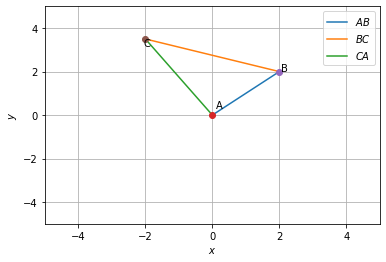
\includegraphics[width=\columnwidth]{Triangle.png}
	\caption{The given points form a triangle}
\end{figure}

\vspace{0.5cm}

From the Fig.1 it is clear that sides BC and AC has same side length, which is different from AB. So the given triangle is not an equilateral triangle.


\vspace{0.5cm}
Here from equations (13),(14) and (15), only two sides of triangle are equal ($\norm{ \vec{A} - \vec{B}} \neq \norm{ \vec{B} - \vec{C}}  = \norm{ \vec{A} - \vec{C}} $).
\textbf{So the given triad of points does not form an equilateral triangle.}

\vspace{0.4cm}

\textbf{Download python code at }
\begin{lstlisting}[frame=single] 
https://github.com/AnishAntony11
/Assignment1
\end{lstlisting}

\end{document}

